\documentclass{article}

\usepackage{fullpage}
\usepackage{listings}
\usepackage{color}
\usepackage{multirow}
\usepackage{tikz}
\usepackage{graphicx}
\usepackage{caption}
\usetikzlibrary{shapes.geometric, arrows}

\tikzstyle{blocked} = [rectangle, rounded corners, minimum width=3cm, minimum height=1cm,text centered, text width=3cm, draw=black, fill=red!30]
\tikzstyle{ready} = [rectangle, rounded corners, minimum width=3cm, minimum height=1cm,text centered, text width=3cm, draw=black, fill=yellow!30]
\tikzstyle{running} = [rectangle, rounded corners, minimum width=3cm, minimum height=1cm,text centered, text width=3cm, draw=black, fill=green!30]
\tikzstyle{io} = [trapezium, trapezium left angle=70, trapezium right angle=110, minimum width=3cm, minimum height=1cm, text centered, draw=black, fill=blue!30]
\tikzstyle{process} = [rectangle, minimum width=3cm, minimum height=1cm, text centered, draw=black, fill=orange!30]
\tikzstyle{decision} = [diamond, minimum width=3cm, minimum height=1cm, text centered, draw=black, fill=green!30]
\tikzstyle{arrow} = [thick,->,>=stealth]

\setlength{\parskip}{0.5em}

\definecolor{dkgreen}{rgb}{0,0.6,0}
\definecolor{gray}{rgb}{0.5,0.5,0.5}
\definecolor{mauve}{rgb}{0.58,0,0.82}

\lstset{
  language=C,
  aboveskip=3mm,
  belowskip=3mm,
  showstringspaces=false,
  columns=flexible,
  basicstyle={\small\ttfamily},
  numbers=none,
  numberstyle=\tiny\color{gray},
  breaklines=true,
  breakatwhitespace=true,
  tabsize=3
}

\title{Pintos Task 1: Scheduling Design Document}
\author{Group 07: Ben Sheng Tan, Adanna Akwataghibe, Mark Aduol, Alessio Incitti }

\begin{document}
\maketitle

\section{PRIORITY SCHEDULING}

\subsection{ DATA STRUCTURES}

\subsection*{A1: (5 marks) }

\textit{Copy here the declaration of each new or changed ‘struct’ or ‘struct’ member, global or static variable, ‘typedef’, or enumeration. Identify the purpose of each in 25 words or less.}
\\ \\
In thread.h, we added:
\begin{lstlisting}
    struct thread
      {
        /* TASK 1 : Priority Checking */
        int base_priority;                /* initial priority of thread */
        struct list_elem donation_thread; /* thread element that is donated */
        struct lock* lock_waiting;        /* lock that thread is waiting for */
        struct list threads_donated;      /* list of threads */

        ...
      };

\end{lstlisting}

Purpose of each new addition:
\\ \\
\texttt{base\_priority}: The base priority of the thread, without taking priority donations into account.

\texttt{donation\_threads}: \texttt{list\_elem} for the donor threads list. The donation thread can be added to another thread's donations

\texttt{lock\_waiting}: Lock that this thread is waiting on.

\texttt{thread\_donated}:  If the \texttt{lock\_waiting} is not NULL, then the current thread is
     waiting for a particular lock. \texttt{thread\_donated} is the list of
     (different) threads which are also waiting for \texttt{lock\_waiting}. This list is ordered by the priority of the threads.


\subsection*{A2: (10 marks) }

\textit{Explain the data structure used to track priority donation. Give a diagram that illustrates a nested donation in your structure.}

Consider 3 threads:

\begin{itemize}
\item Thread T1, initial priority 31.
\item Thread T2, initial priority 32.
\item Thread T3, initial priority 33.
\end{itemize}

Now assume that the threads execute as follows.

\begin{center}
T1 = \{\ldots down(L1) \ldots up(L1) \ldots \}
\end{center}
\begin{center}
T2 = \{\ldots down(L2) \ldots down(L1) \ldots up(L1) \ldots up(L2) \ldots \}
\end{center}
\begin{center}
T3 = \{\ldots down(L2) \ldots up(L2) \ldots \}
\end{center}

Assume that at time \textit{t0}, threads \texttt{T1} and \texttt{T2} have acquired locks \texttt{L1} and \texttt{L2} respectively. At time \textit{t1}, thread \texttt{T3} begins running. At time \textit{t2}, thread \texttt{T3} attempts to acquire lock \texttt{L2} but is prevented from doing so since lock \texttt{L2} has already been acquired by thread \texttt{T2}. But since \texttt{T3} has a higher priority than \texttt{T2}, \texttt{T3} donates it's priority to \texttt{T2}. Priority donation work as follows.

\begin{enumerate}
\item The \texttt{lock\_waiting} member of \texttt{T3}'s thread \texttt{struct} is initialised to lock \texttt{L2}.
\item By using the \texttt{list\_elem} \texttt{donation\_thread} member of \texttt{struct thread}, \texttt{T3} is inserted into the \texttt{donated\_threads} list of \texttt{T2}, in descending order of priority, using the comparator \texttt{is\_lower\_priority}.
\item We then call \texttt{sema\_down()} to put \texttt{T3} to sleep.
\item However, before \texttt{T3} is actually blocked, we call \texttt{donate\_priority()} to donate thread \texttt{T3}'s priority to the thread holding lock \texttt{L2} - which is \texttt{T2}.
\item Thread \texttt{T3} is then inserted at the back of the list of waiters on the \texttt{L2}'s semaphore and blocked.
\item The thread with the next highest priority, \texttt{T2} is then run and eventually performs the same operations, with respect to lock \texttt{L1}.
\item When thread \texttt{T1} runs (as the other two threads with higher priorities are blocked) it wille eventually release lock \texttt{L1}. Upon doing so, \texttt{T1}'s priority is reset to the priority it had upon acquisition of lock \texttt{L1}.
\item Upon lowering it's priority, \texttt{T1} is blocked and and \texttt{T2} is run. Similarly, when \texttt{T2} releases lock \texttt{L2} and releases it's inherited priority (that is, lower it's priority down to that which it had upon acquisition of \texttt{L2}), \texttt{T3} preempts \texttt{T2} and \texttt{T3} continues its execution.
\end{enumerate}

\newpage
The following depicts the changes in thread state as priorities are donated, with respect to time. Red blocks denote blocked threads; yellow blocks denote threads on the ready queue and the green block denotes the running thread.
\\\\

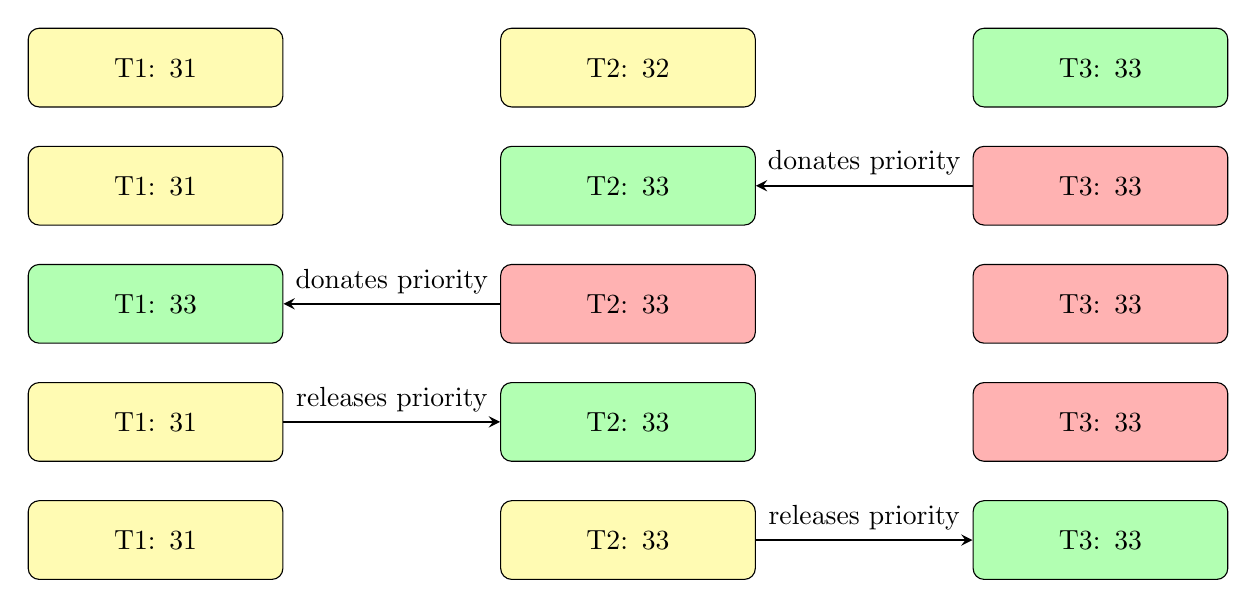
\begin{tikzpicture}[node distance=2cm]
\node (startA) [ready] {T1: 31};
\node (startB) [ready, right of=startA, xshift=4cm] {T2: 32};
\node (startC) [running, right of=startB, xshift=4cm] {T3: 33};

\node (startA1) [ready, below of=startA, yshift=0.5cm] {T1: 31};
\node (startB1) [running, below of=startB, yshift=0.5cm] {T2: 33};
\node (startC1) [blocked, below of=startC, yshift=0.5cm] {T3: 33};
\draw [arrow] (startC1) -- node[anchor=south] {donates priority} (startB1);

\node (startA2) [running, below of=startA1, yshift=0.5cm] {T1: 33};
\node (startB2) [blocked, below of=startB1, yshift=0.5cm] {T2: 33};
\node (startC2) [blocked, below of=startC1, yshift=0.5cm] {T3: 33};
\draw [arrow] (startB2) -- node[anchor=south] {donates priority} (startA2);

\node (startA3) [ready, below of=startA2, yshift=0.5cm] {T1: 31};
\node (startB3) [running, below of=startB2, yshift=0.5cm] {T2: 33};
\node (startC3) [blocked, below of=startC2, yshift=0.5cm] {T3: 33};
\draw [arrow] (startA3) -- node[anchor=south] {releases priority} (startB3);

\node (startA4) [ready, below of=startA3, yshift=0.5cm] {T1: 31};
\node (startB4) [ready, below of=startB3, yshift=0.5cm] {T2: 33};
\node (startC4) [running, below of=startC3, yshift=0.5cm] {T3: 33};
\draw [arrow] (startB4) -- node[anchor=south] {releases priority} (startC4);
\end{tikzpicture}

\begin{figure}
\centering
\captionsetup{justification=centering}

\includegraphics[width=\linewidth]{nested_donation_diagram.png}
\caption{Shows how nested priority donation is implemented. Curved arrows denote a pointer from one thread to another.}
\label{fig:diagram}
\end{figure}




\subsection{ALGORITHMS}

\subsubsection*{A3: (5 marks) }
\textit{How do you ensure that the highest priority thread waiting for a lock, semaphore, or condition variable wakes up first?}
\\ \\
For locks and semaphores, this is handled by sorting the waiters list by the priority of the threads. For example, when a thread goes to sleep on some lock or semaphore, \texttt{sema}, it is added to the list \texttt{\&sema->waiters} or \texttt{\&lock->waiters}. One of the invariants maintained on these list is that their elements - the threads waiting on the or lock semaphore - are always sorted in descending order of priority. This invariant is maintained by always adding elements to the list using the \texttt{list\_insert\_ordered} function, and passing the comparator, \texttt{is\_lower\_priority} as the necessary, element comparison function. A thread is woken up by popping the first element off the lock's or semaphore's waiters list, so unblocking it. For condition variables, since each semaphore in the list of waiters has exactly one thread, it is sorted in increasing order of priority of the thread in each semaphore and the semaphore to call \texttt{sema\_up} on is also the first element in its waiters list.
\\ \\

\subsubsection*{A4: (5 marks) }
\textit{Describe the sequence of events when a call to \texttt{lock\_acquire()} causes a priority donation. How is nested donation handled?}
\\ \\
The \texttt{lock\_acquire} function first checks whether the basic, priority donation policy is enabled and whether the lock in question has already been acquired by another thread. If both these conditions hold, then the \texttt{lock\_waiting} field of the current thread is assigned the value \texttt{lock} - where \texttt{lock} is simply a pointer to the lock in question. The current thread - through its \texttt{donation\_thread} field - is then inserted into the \texttt{threads\_donated} list of the thread currently holding the lock. This insertion is actually an ordered insertion, using the comparator \texttt{is\_lower\_priority} to maintain the invariant that list of waiting threads is sorted in ascending order of priority. Both \texttt{donation\_thread} and \texttt{threads\_donated} are stored in \texttt{struct thread}.
After calling \texttt{sema\_down}, the current thread's \texttt{wait\_lock} is reset to \texttt{NULL}.
To handle nested donation, \texttt{donate\_priority()} declares a new struct thread and lock for its execution. This function checks if the current thread has a donee by using the \texttt{lock\_waiting} field. If it does have one, that threads \texttt{threads\_donated} is reordered using \texttt{update\_priority()}. This function updates the priority member in thread struct with the effective priority (i.e. taking into account donations).
\\\\

\subsubsection*{A5: (5 marks) }
\textit{Describe the sequence of events when \texttt{lock\_release()} is called on a lock that a higher-priority thread is waiting for.}
\\ \\
Upon a call of \texttt{lock\_release()}, after checking that advanced scheduler mode is off (\texttt{thread\_mlfqs = false}), a call to \texttt{remove\_with\_lock(lock)} is executed passing the lock as argument. This function removes every item from the list \texttt{threads\_donated} which is waiting for lock l.
Note that since the lock waiters list is ordered (as mentioned in A3) we can assume that the new owner of the lock will be the first element of this list. As such, we donate the priority of all other waiters in the list to its first element.
Then, back to the \texttt{lock\_release()} context, \texttt{update\_priority} is called. This changes the priority of the current thread only if the priority of the first element of the \texttt{threads\_donated} is greater than its current priority, so it will change the priority to the first elements priority. Since list \texttt{threads\_donated} is sorted highest to lowest priority, now the current thread has the highest priority of all the \texttt{threads\_donated} (except for the first element which it is equal to).
Finally, \texttt{sema\_up} is called which unblocks the first element of the waiters list.
\\ \\


\subsection{SYNCHRONIZATION}

\subsubsection*{A6: (5 marks) }
\textit{Describe a potential race in \texttt{thread\_set\_priority()} and explain how your implementation avoids it.  Can you use a lock to avoid this race?}
\\ \\
A potential race in \texttt{thread\_set\_priority()} is that in (line A6a) we have that the current thread is setting its base priority to new priority and there could be an interrupt before we call \texttt{update\_priority()}, which would mean that the thread's base priority is not updated properly. We disable interrupts in order to avoid this race condition. We cannot use locks in this situation as the interrupt could still happen before \texttt{update\_priority()} is called.
\\ \\
In thread.c, we added:
\begin{lstlisting}
    void thread_set_priority (int new_priority)
    {
      /* Advanced scheduler mode makes no use of this function */
      if(thread_mlfqs) return;

      enum intr_level level = intr_disable();
      int priority_prev = thread_current()->priority;
      thread_current()->base_priority = new_priority;                                   (Line A6a)
      update_priority();

      if(priority_prev < thread_current()->priority) {
        donate_priority();
      }
      if (priority_prev > thread_current()->priority) {
        check_max_priority();
      }

      intr_set_level(level);
    }
\end{lstlisting}


\subsection{RATIONALE}

\subsubsection*{A7: (5 marks) }
\textit{Why did you choose this design?  In what ways is it superior to another design you considered?}
\\ \\
We chose to use interrupts most of the time, instead of locks because it made the code clearer and it was a good way to make sure that in a block of code which was updating a value of the thread, that only one thread would be running and we would not have any races.
The reason why we decided to used a priority-based sorted ready\_list is because it makes it much more efficient for the function check\_max\_priority to check against the list since it can be assumed that the front has the highest priority, therefore it requires constant time. However, a disadvantage to this is that insertion into the list has higher cost because list\_insert\_ordered is used instead of list\_push\_back, which in the worst case requires a comparison against every element of the list. We believe that this design is superior to a non-sorted ready\_list because it is overall more efficient and much clearer conceptually.

\section{ADVANCED SCHEDULER}

\subsection{DATA STRUCTURES}

\subsection*{B1: (5 marks) }

\textit{Copy here the declaration of each new or changed ‘struct’ or ‘struct’ member, global or static variable, ‘typedef’, or enumeration. Identify the purpose of each in 25 words or less.}
\\\\
In thread.h, we added:
\begin{lstlisting}
    struct thread
      {
        ...
        /* TASK 1: Advanced scheduling */
        int cpu_num;
        int nice;
        ...
        };
\end{lstlisting}

In 'thread.c', we added:
\begin{lstlisting}
    static int load_avg;
\end{lstlisting}

Purpose of each new addition:

\texttt{int cpu\_num}: the recent CPU value of the current thread in fixed point.

\texttt{int nice}: niceness value of the current thread.

\texttt{int load\_avg}: the system's load average value in fixed point.


\subsection{ALGORITHMS}

\subsubsection*{B2: (5 marks) }
\textit{Suppose threads A, B, and C have nice values 0, 1, and 2.  Each has a \texttt{recent\_cpu} value of 0.  Fill in the table below showing the scheduling decision and the priority and \texttt{recent\_cpu} values for each thread after each given number of timer ticks:}

\begin{table}[htb]
\centering
\begin{tabular}{llllllll}
\multirow{2}{*}{\begin{tabular}[c]{@{}c@{}}timer\\ ticks\end{tabular}} & \multicolumn{3}{c|}{recent\_cpu} & \multicolumn{3}{c|}{priority} & thread to run \\ \cline{2-8}
                                                                       & A         & B         & C       & A        & B        & C       &               \\ \hline
                                                                       0           & 0         & 0       & 0        & 63       & 61       & 59      & A             \\ \hline
                                                                       4           & 4         & 0       & 0        & 62       & 61       & 59      & A             \\ \hline
                                                                       8           & 8         & 0       & 0        & 61       & 61       & 59      & B             \\ \hline
                                                                       12          & 8         & 4       & 0        & 61       & 60       & 59      & A            \\ \hline
                                                                       16          & 12        & 4       & 0        & 60       & 60       & 59      & B             \\ \hline
                                                                       20          & 12        & 8       & 0        & 60       & 59       & 59      & A             \\ \hline
                                                                       24          & 16        & 8       & 0        & 59       & 59       & 59      & C             \\ \hline
                                                                       28          & 16        & 8       & 4        & 59       & 59       & 58      & B            \\ \hline
                                                                       32          & 16        & 12      & 4        & 59       & 58       & 58      & A             \\ \hline
                                                                       36          & 20        & 12      & 4        & 58       & 58       & 58      & C             \\ \hline
                                                                       \end{tabular}
\end{table}

\subsubsection*{B3: (5 marks) }
\textit{Did any ambiguities in the scheduler specification make values in the table uncertain?  If so, what rule did you use to resolve them?  Does this match the behaviour of your scheduler?}
\\ \\
They were some ambiguities in the scheduler specification. For example,it does not specify what happens what thread is supposed to run if multiple threads all have the same priority. We are not told which thread is supposed to run in this instance.
  \\\\
In order to solve this problem, we use both the Round Robin and FIFO (first in, first out) rules which is what our scheduler implements as well.
  \\\\
For the FIFO implementation, the \texttt{ready\_list} contains all the threads which are ready to run. So, if the scheduler needs to choose between multiple threads to run, it simply chooses the first thread in the \texttt{ready\_list}, which by default is the thread who has the lowest running time.
  \\\\
For the Round Robin implementation, if the current (running) thread has the same priority as a ready thread, and this priority also happens to be the highest priority, then when the current thread reaches the \texttt{TIME\_SLICE} (4 ticks), it continues running regardless.

\subsubsection*{B4: (5 marks) }
\textit{How is the way you divided the cost of scheduling between code inside and outside interrupt context likely to affect performance?}
\\ \\
Since the load average, cpu and priority of mlfqs all have to be calculated after a set amount of time (we are given that the load average and cpu have to be calculated every one second and the thread priority has to recalculated every 4 ticks), it is therefore neccessary to have these calculations in the timer interrupt handler. However, it would be more efficient if the calculations were not done in the interrupt handler because the thread that is interrupted would have less running time and it would stop the running of other interrupts as well. So with more threads that are interrupted, the more performance is affected.

\subsection{RATIONALE}

\subsubsection*{B5: (5 marks) }
\textit{Briefly critique your design, pointing out advantages and disadvantages in your design choices.}
\\ \\
 Calculating the load average, the cpu and the derived thread priority in the
  timer interrupt handler will allow the scheduler to be more dynamic as it can
  keep up to date with what is happening every certain number of ticks (4 in this case).
  On the other hand this will severely slow down performance since the timer interrupt
  handler gets called constantly and therefore there is a large amount of computation
  executed frequently.
Other disadvantages affecting performance are the lack of use of locks in our code - which in some cases could make it inefficient when running threads - and the fixed point function definitions: it may have been faster if the fixed point functions were implemented as macros rather than functions, since we are only using them in the one file. On the upside, these design choices have the advantage of clarity.
\\ \\

\subsubsection*{B6: (5 marks) }
\textit{The assignment explains arithmetic for fixed-point mathematics in detail, but it leaves it open to you to implement it.  Why did you decide to implement it the way you did?  If you created an abstraction layer for fixed-point mathematics, that is, an abstract data type and/or a set of functions or macros to manipulate fixed-point numbers, why did you do so?  If not, why not?}
\\ \\
We created one header file for the implementations of fixed point arithmetic: \texttt{fixedpointrealarith.h}, which includes functions that perform the calculations needed.
We chose to implement it like this for the following reasons:

    - Easy to call the functions to calculate in thread.c
    
	- Each function name was given clearly for example \texttt{div\_x\_y} and \texttt{div\_x\_n}
	  where in each function name, x and y would represent fixed-point numbers
	  and n would represent an integer.
      
	- If for any reason, an error was made in the implementation of the function
      since we only wrote the calculations once, it was easy to change the offending
      function (since it was only in the .h file).

\end{document}
